The normal vectors of the planes are 
\begin{equation}
 \vec n_1=\myvec{2\\1\\3},
 \vec n_2 =\myvec{1\\-2\\5},
\end{equation} respectively.
Consequently, the angle between the planes is 
%
\begin{align}
    \cos\theta &= \frac{\vec{n_1^\top}\vec{n_2}}{\norm {\vec{n_1}}\norm{\vec{n_2}}}\\
&==\sqrt{\frac{15}{28}}
    \label{linform/43/b/eq9}
\end{align} 
$\therefore$ the planes  are neither parallel nor perpendicular, as can be verfied from 
Fig. \ref{linform/43/b/fig:1}.
%
\begin{figure}[!ht]
\centering
    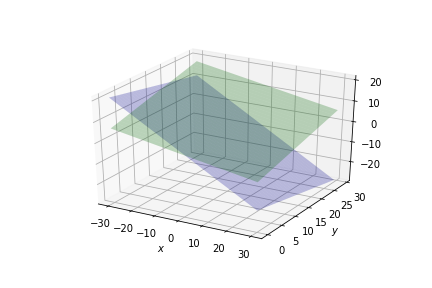
\includegraphics[width= \columnwidth]{solutions/su2021/2/43/b/assignment4.png}
    \caption{Planes $P_1$ and $P_2$} \label{linform/43/b/fig:1}
\end{figure}
